% Generative Compression for Differentiable Opaque Meshes -- technical report
% VERSION: report-latex-v4 (2026-11-05 evening): v3 + Section 2.8 filled (lambda x dictionary fan: Table 6, Figure 7) + Section 2.9 indoor top-rate loss decomposition (Table 7) + open list updated. Base: report-latex-v3 (2026-11-05): every comment of Yao's 11/05 review addressed (plan/advisor-report-comments-2026-11-05.md): price calibration, lambda vs size, collapse/Euler, codec details (edge cache, 1-ring context, DC, banks, five streams), mean RD curve figure, Table 2 as (MB (ratio), dPSNR), Fig 4 panel (a) only, 3DGS-class figure/table moved to the appendix, lambda x dictionary fan placeholder (Table X). Compile with pdflatex.
\documentclass[11pt,a4paper]{article}
\usepackage[margin=2.2cm]{geometry}
\usepackage[T1]{fontenc}
\usepackage[utf8]{inputenc}
\usepackage{lmodern}
\usepackage{amsmath,amssymb}
\usepackage{graphicx}
\usepackage{booktabs}
\usepackage{array}
\usepackage{xcolor}
\usepackage{caption}
\usepackage{tikz}
\usetikzlibrary{arrows.meta,positioning,calc,fit}
\usepackage{enumitem}
\usepackage[colorlinks=true,linkcolor=blue!60!black,citecolor=blue!60!black,urlcolor=blue!60!black]{hyperref}

\captionsetup{font=small,labelfont=bf}
\definecolor{ours}{RGB}{31,119,80}
\definecolor{oursfill}{RGB}{229,243,236}
\definecolor{edge}{RGB}{90,90,90}
\definecolor{quiet}{RGB}{110,110,110}

\newcommand{\MB}{\,\mathrm{MB}}
\newcommand{\dB}{\,\mathrm{dB}}

\title{Generative Compression for Differentiable Opaque Meshes\\[2pt]
\large Technical report}

\begin{document}
\maketitle

\begin{abstract}
MeshSplatting produces an opaque, engine-ready triangle mesh with per-vertex spherical harmonics (SH), but its FP32 output is 430--740\,MB per scene. We keep MeshSplatting's optimisation untouched and add two training-time decisions and one delivery codec: triangles are split only when the distortion they remove is worth the bytes they add, the same price is applied in reverse as an edge-collapse prune, and the trained mesh is encoded into a single file whose per-vertex SH is replaced by shared dictionary indices. One rate--distortion parameter $\lambda$ traces the whole curve. On Mip-NeRF~360 the 642\,MB FP32 mesh becomes 26.6\,MB at $-0.24$\,dB (24$\times$), 9.0\,MB at $-0.92$\,dB (72$\times$) and 4.3\,MB at $-1.68$\,dB (151$\times$); the delivered asset is a standard mesh that decodes in 2--6\,s on one CPU core and renders at 145--350\,fps on a phone.
\end{abstract}

% =====================================================================
\section{Methodology}
\label{sec:method}

We keep MeshSplatting's optimisation untouched and change two things: \emph{which} triangles get split during growth (priced in bytes), and a reverse prune under the same price. The trained mesh then goes through a codec that replaces per-vertex SH by shared dictionary indices. The vertex count is no longer a hand-set cap but an output of one rate--distortion trade-off $\lambda$. Figure~\ref{fig:pipeline} shows where the pieces sit.

\begin{figure}[t]
\centering
\resizebox{\linewidth}{!}{%
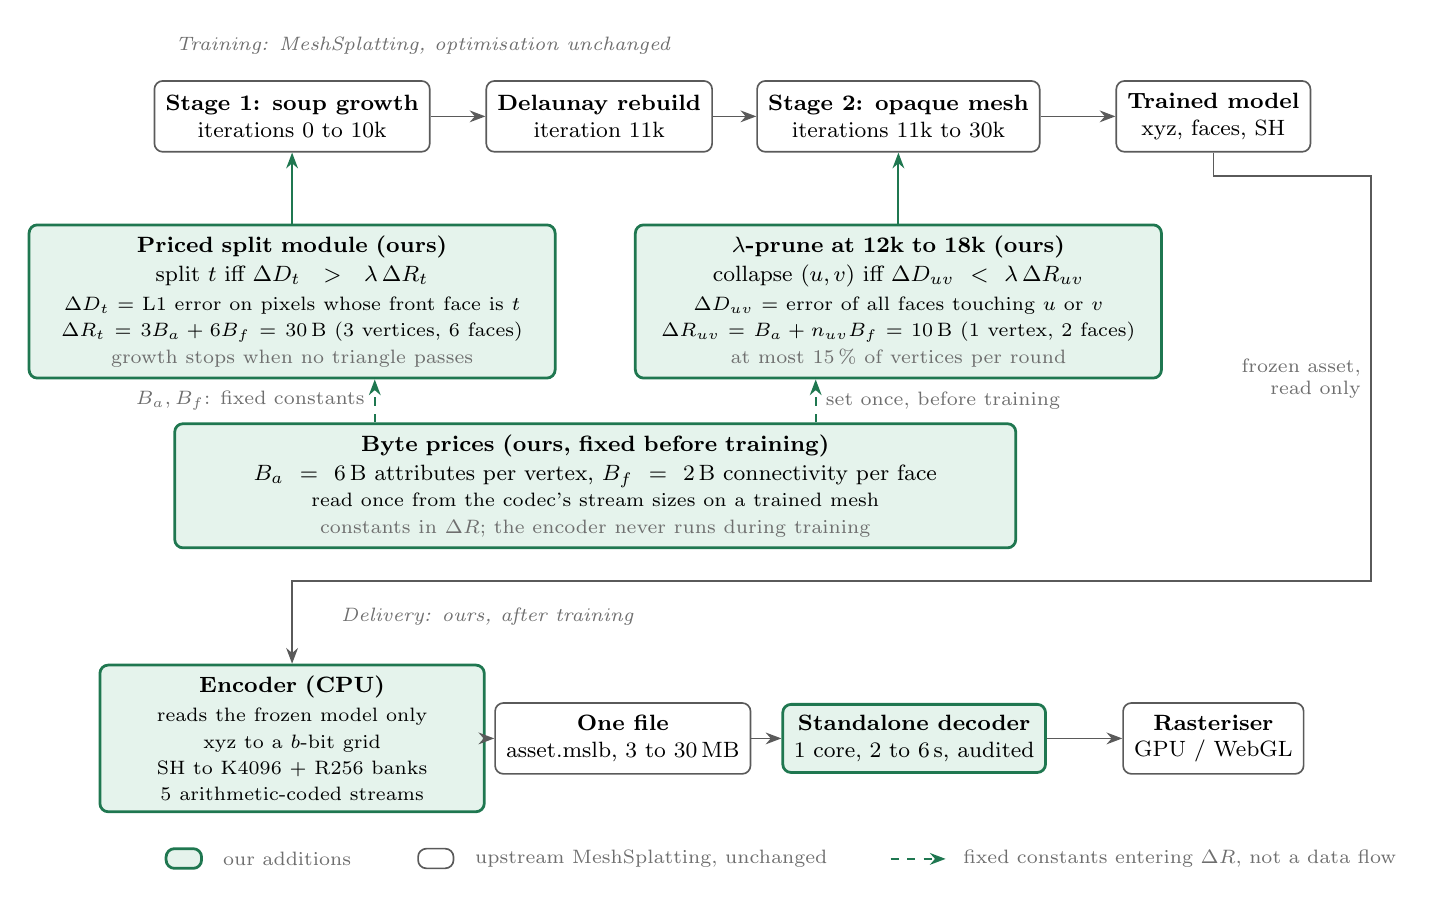
\begin{tikzpicture}[
  font=\footnotesize,
  >={Stealth[length=2mm]},
  up/.style={draw=edge, rounded corners=3pt, line width=0.6pt, align=center, inner sep=4pt, minimum height=9mm},
  ourbox/.style={draw=ours, fill=oursfill, rounded corners=3pt, line width=1.0pt, align=center, inner sep=4pt},
  flow/.style={->, draw=edge, line width=0.6pt},
  ourflow/.style={->, draw=ours, line width=0.7pt},
  price/.style={->, draw=ours, dashed, line width=0.7pt},
  lane/.style={font=\scriptsize\itshape, text=quiet},
  body/.style={font=\scriptsize, text=black},
]
% ---- lane 1: upstream training
\node[lane, anchor=west] at (0,0.9) {Training: MeshSplatting, optimisation unchanged};
\node[up] (s1) at (1.6,0) {\textbf{Stage 1: soup growth}\\ iterations 0 to 10k};
\node[up] (del) at (5.5,0) {\textbf{Delaunay rebuild}\\ iteration 11k};
\node[up] (s2) at (9.3,0) {\textbf{Stage 2: opaque mesh}\\ iterations 11k to 30k};
\node[up] (model) at (13.3,0) {\textbf{Trained model}\\ xyz, faces, SH};
\draw[flow] (s1) -- (del);
\draw[flow] (del) -- (s2);
\draw[flow] (s2) -- (model);

% ---- lane 2: our priced decisions
\node[ourbox, below=9mm of s1.south, anchor=north, text width=6.4cm] (split) {
  \textbf{Priced split module (ours)}\\[1pt]
  split $t$ iff $\Delta D_t > \lambda\,\Delta R_t$\\[1pt]
  {\scriptsize $\Delta D_t$ = L1 error on pixels whose front face is $t$}\\
  {\scriptsize $\Delta R_t = 3B_a + 6B_f = 30$\,B (3 vertices, 6 faces)}\\
  {\scriptsize\color{quiet} growth stops when no triangle passes}};
\node[ourbox, below=9mm of s2.south, anchor=north, text width=6.4cm] (prune) {
  \textbf{$\lambda$-prune at 12k to 18k (ours)}\\[1pt]
  collapse $(u,v)$ iff $\Delta D_{uv} < \lambda\,\Delta R_{uv}$\\[1pt]
  {\scriptsize $\Delta D_{uv}$ = error of all faces touching $u$ or $v$}\\
  {\scriptsize $\Delta R_{uv} = B_a + n_{uv}B_f = 10$\,B (1 vertex, 2 faces)}\\
  {\scriptsize\color{quiet} at most 15\,\% of vertices per round}};
\draw[ourflow] (split.north) -- (s1.south);
\draw[ourflow] (prune.north) -- (s2.south);

% ---- price table
\node[ourbox, text width=10.4cm] (price) at ($(split.south)!0.5!(prune.south) + (0,-1.35)$) {
  \textbf{Byte prices (ours, fixed before training)}\\[1pt]
  $B_a = 6$\,B attributes per vertex, $B_f = 2$\,B connectivity per face\\
  {\scriptsize read once from the codec's stream sizes on a trained mesh}\\
  {\scriptsize\color{quiet} constants in $\Delta R$; the encoder never runs during training}};
\draw[price] ([xshift=-2.8cm]price.north) -- ([xshift=-2.8cm]price.north |- split.south) node[midway, left, body, text=quiet] {$B_a, B_f$: fixed constants};
\draw[price] ([xshift=2.8cm]price.north) -- ([xshift=2.8cm]price.north |- prune.south) node[midway, right, body, text=quiet] {set once, before training};

% ---- lane 3: delivery
\node[lane, anchor=west] at (2.1,-6.35) {Delivery: ours, after training};
\node[ourbox, text width=4.6cm] (enc) at (1.6,-7.9) {
  \textbf{Encoder (CPU)}\\[1pt]
  {\scriptsize reads the frozen model only}\\
  {\scriptsize xyz to a $b$-bit grid}\\
  {\scriptsize SH to K4096 + R256 banks}\\
  {\scriptsize 5 arithmetic-coded streams}};
\node[up] (file) at (5.8,-7.9) {\textbf{One file}\\ asset.mslb, 3 to 30\,MB};
\node[ourbox] (dec) at (9.5,-7.9) {\textbf{Standalone decoder}\\ 1 core, 2 to 6\,s, audited};
\node[up] (ras) at (13.3,-7.9) {\textbf{Rasteriser}\\ GPU / WebGL};
\draw[flow] (enc) -- (file);
\draw[flow] (file) -- (dec);
\draw[flow] (dec) -- (ras);
\draw[flow] (model.south) -- ++(0,-0.3) -| (15.3,-5.9) node[pos=0.75, left, body, text=quiet, align=right] {frozen asset,\\ read only} -- (1.6,-5.9) -- (enc.north);

% ---- key
\begin{scope}[shift={(0,-9.55)}]
\draw[ourbox, minimum width=4mm, minimum height=2.5mm] (0,0) rectangle (0.45,0.25);
\node[body, text=quiet, anchor=west] at (0.6,0.12) {our additions};
\draw[up, minimum width=4mm] (3.2,0) rectangle (3.65,0.25);
\node[body, text=quiet, anchor=west] at (3.8,0.12) {upstream MeshSplatting, unchanged};
\draw[price] (9.2,0.12) -- (9.9,0.12);
\node[body, text=quiet, anchor=west] at (10.0,0.12) {fixed constants entering $\Delta R$, not a data flow};
\end{scope}
\end{tikzpicture}}
\caption{Pipeline: two priced decisions during training, one dictionary codec at delivery. Grey boxes are MeshSplatting as published; tinted boxes are ours. The byte prices are two constants read once from the codec's stream sizes; the encoder itself runs only on the frozen, finished model and cannot influence how the mesh grew.}
\label{fig:pipeline}
\end{figure}

\subsection{Where we intervene in MeshSplatting}

Upstream training has two stages. \textbf{Stage 1 (iterations 0--10\,000)} grows a soft triangle soup: every 500 iterations a fixed fraction of triangles (\texttt{add\_percentage}) is split, chosen by importance sampling, up to a hand-set cap. At iteration 11\,000 a restricted Delaunay rebuild re-triangulates the soup. \textbf{Stage 2 (11\,000--30\,000)} optimises the now-opaque mesh (opacity schedule, $2\times$/$4\times$ supersampling after 20k/25k).

Our changes sit only in the growth decisions:
\begin{enumerate}[nosep,leftmargin=*]
  \item \textbf{Stage 1, the split rule.} The importance-sampled split is replaced by a priced one: a triangle is split only if the distortion it would remove is worth the bytes it adds (Section~\ref{sec:rate}). Growth stops by itself when no triangle passes.
  \item \textbf{Stage 2, $\lambda$-prune rounds} at iterations 12k / 14k / 16k / 18k (after the Delaunay rebuild, before supersampling): edges whose faces carry too little residual for the bytes they cost are collapsed, at most 15\,\% of the vertices per round, with a fold-over guard. Same $\lambda$, applied in reverse.
\end{enumerate}
Losses, learning rates, opacity schedule, Delaunay rebuild, supersampling and final cleaning are upstream code imported as is. The appearance optimisation is MeshSplatting's own.

\subsection{How the rate cost is estimated and used}
\label{sec:rate}

\paragraph{Distortion.} For every triangle $t$ we accumulate during each densification interval its \textbf{distortion mass} $\Delta D_t$: the per-pixel L1 error summed over the pixels whose front-most triangle is $t$ (from the rasteriser's per-pixel triangle ids), divided by the megapixels of the image and averaged over the training views of the interval. A triangle that is visible in more views, covers more pixels, or is rendered worse carries more mass. The prune uses the same per-triangle quantity $\Delta D_t$, summed over the triangles around an edge.

\paragraph{Rate.} Rate is counted in bytes of the delivered file, from two constants:
\begin{itemize}[nosep,leftmargin=*]
  \item $B_a = 6$\,B, the \emph{attribute} bytes of one vertex: quantised position residual ($\approx 2.3$\,B), DC colour ($\approx 1.5$\,B) and its two SH dictionary indices ($\approx 2.4$\,B);
  \item $B_f = 2$\,B, the \emph{connectivity} bytes of one face.
\end{itemize}
A file with $V$ vertices and $F$ faces therefore costs $V B_a + F B_f$ bytes plus a fixed 0.6\,MB of dictionaries and header. Neither constant contains the other. The constants are not learned: they are the measured stream sizes of our own lossless coder (Section~\ref{sec:codec}) on one delivered Room asset, divided by its vertex and face counts (positions 2.3\,B, DC 1.5\,B, two dictionary indices 2.4\,B per vertex; connectivity 31.7\,bit per vertex $\approx 2$\,B per face at two faces per vertex), fixed before training and reused for every scene and every $\lambda$. The true cost does drift with the operating point: over the 44 delivered assets it is 9.5--13.3\,B per vertex (median 10.8 against the 10\,B the constants imply), rising slightly with $\lambda$ because sparser meshes have longer edges and fewer edge-cache hits. Since the rules below compare $\Delta D / \Delta R$ with $\lambda$, a price error of a factor $c$ is identical to using $c\lambda$; the observed $\pm 30\,\%$ is less than a quarter of one step of our $\lambda$ grid, so it moves the operating point slightly along the same curve rather than changing the curve.

\paragraph{The two rules.} Every mesh edit is a discrete decision in the Lagrangian $J = D + \lambda R$ and is accepted iff it lowers $J$:
\begin{align}
\text{split } t &\iff \frac{\Delta D_t}{\Delta R_t} > \lambda, & \Delta R_t &= 3B_a + 6B_f, \label{eq:split}\\
\text{collapse } (u,v) &\iff \frac{\Delta D_{uv}}{\Delta R_{uv}} < \lambda, & \Delta D_{uv} &= \sum_{f \in N(u)\,\cup\,N(v)} \Delta D_f, \quad \Delta R_{uv} = B_a + n_{uv} B_f , \label{eq:collapse}
\end{align}
where $N(u)$ is the set of faces that have $u$ as a corner and $n_{uv}$ the number of faces that contain the edge $(u,v)$.
\begin{itemize}[nosep,leftmargin=*]
  \item \textbf{Split.} Subdividing $t$ at its three edge midpoints adds three vertices. The stage-1 faces are discarded at the Delaunay rebuild; for a closed triangle mesh Euler's formula gives $F \approx 2V$, and our delivered meshes have 1.8--3.4 faces per vertex (median 2.3), so each added vertex is charged two faces: $\Delta R_t = 3B_a + 6B_f = 30$\,B. $\Delta D_t$ is an upper bound on the error a split can remove.
  \item \textbf{Collapse.} One collapse merges $u$ and $v$ into their midpoint: one vertex and the $n_{uv}$ faces on the edge disappear ($n_{uv} = 2$ for an interior edge, 1 on a boundary), so $\Delta R_{uv} = B_a + n_{uv}B_f = 10$\,B for an interior edge. $\Delta D_{uv}$ is the error of every face whose shape the collapse changes, i.e.\ the union of the two vertex rings; a ring with little error is one the remaining optimisation can repair. A prune round applies many collapses, in increasing order of $\Delta D_{uv}/\Delta R_{uv}$, on an independent set of edges (no two share a vertex), skipping collapses that would fold a surviving face, up to 15\,\% of the vertices per round.
\end{itemize}
Figure~\ref{fig:splitprune} works through one split and one collapse with numbers. $\lambda$ is in units of L1 mass per byte. Four values ($6.2\times10^{-4}$, $1.85\times10^{-3}$, $6.2\times10^{-3}$, $1.85\times10^{-2}$) trace the RD curve; one $\lambda$ stops growth at 15--100\,\% of the dense vertex count depending on the scene, i.e.\ the budget adapts to scene content.

\paragraph{Choosing $\lambda$.} $\lambda$ is the Lagrange multiplier, as in the $\lambda$-mode rate control of video codecs and in HAC / RDO-Gaussian: it fixes the marginal slope, not the size, and the size decreases monotonically with $\lambda$. We have no closed form; empirically $\log(\text{size})$ is close to linear in $\log\lambda$ with slope $\approx -0.6$ on every scene (Table~\ref{tab:perscene}: room 22.1 $\to$ 2.9\,MB, garden 36.4 $\to$ 5.0, kitchen 24.5 $\to$ 3.8 over a 30$\times$ range of $\lambda$), so a target size is reached by one interpolation on that law or one short calibration run. The alternative, stopping growth at a byte budget, is our ``train-at-budget'' ablation (Section~\ref{sec:ablation}); it hits a size exactly but gives each scene a different marginal slope, whereas one $\lambda$ is the same exchange rate everywhere.

\begin{figure}[t]
\centering
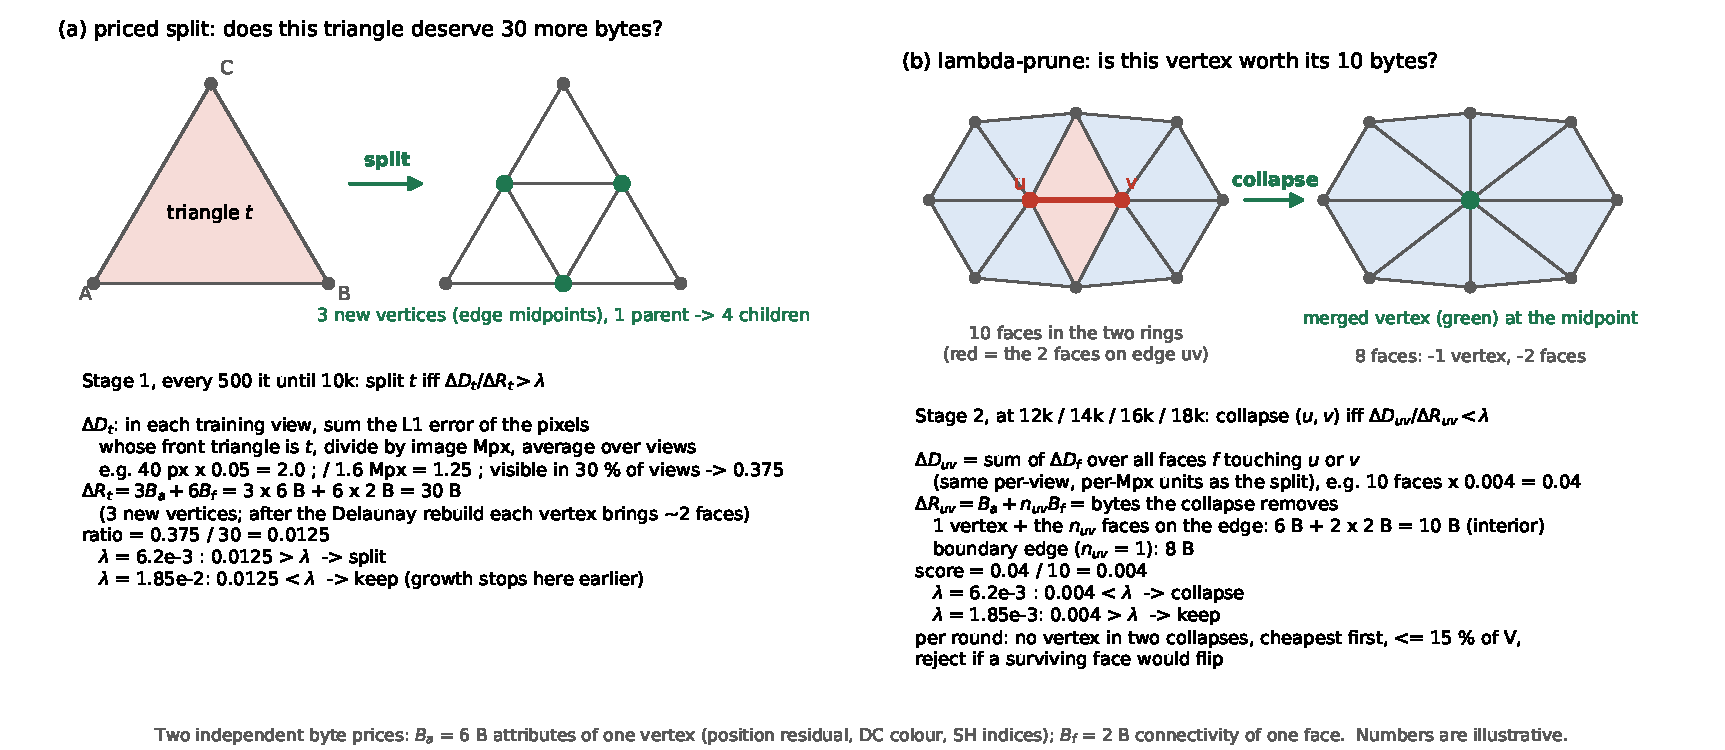
\includegraphics[width=\linewidth]{figures/fig-split-prune-v2.pdf}
\caption{One priced split (a) and one $\lambda$-collapse (b), with illustrative numbers. Both use the same $\lambda$, the same per-face distortion and the same two byte prices $B_a$, $B_f$.}
\label{fig:splitprune}
\end{figure}

\paragraph{Why constants.} $B_a$ and $B_f$ were calibrated once on one asset and then frozen: they are inputs to training, not outputs of it. Measured afterwards on all 44 delivered assets the true cost is 9.5--13.3\,B per vertex against the 10\,B the constants imply, and a price error of a factor $c$ is equivalent to using $c\lambda$, i.e.\ it shifts the operating point along the curve by less than a quarter of a grid step. A per-scene price would buy nothing but would make $\lambda$ a different exchange rate in every scene.

\textbf{The encoder is not in the training loop.} Its only contribution to training is these two constants; $\Delta R$ is computed from them, never by encoding anything during training. The encoder itself runs once, after iteration 30k, on the frozen model, and cannot influence how the mesh grew.

\subsection{Encoder and decoder}
\label{sec:codec}

The encoder takes the finished mesh (positions, faces, 48 SH coefficients per vertex, per-vertex opacity) and writes one file of five entropy-coded streams plus a small header. The lossy steps (SH dictionary assignment, position and DC quantisation, one opacity constant) all happen before the streams; the streams themselves are lossless and the encoder verifies a byte-exact round trip before writing.
\begin{enumerate}[nosep,leftmargin=*]
  \item \textbf{Connectivity.} Faces are visited in a cache-friendly strip order (meshoptimizer). The decoder keeps a ring buffer of the 64 most recently decoded \emph{directed} edges. For each triangle the encoder writes either \emph{hit} (the triangle shares an edge with the buffer: one flag, the buffer slot and the third vertex) or \emph{miss} (three vertices). A vertex seen for the first time is written as a single zero symbol, its id being implicitly the next unused one, so no vertex order is transmitted; a known vertex is written as the zigzag difference to the last id. All symbols go through an adaptive binary arithmetic coder~\cite{witten1987} with $5\times 256$ contexts and no transmitted tables, in the spirit of the mesh buffer of Deering~\cite{deering1995}. The stream costs $\approx 15$\,bit per triangle (66 raw). Edgebreaker-class coders ($\approx 2$\,bit per triangle on manifold meshes) do not apply directly to MeshSplatting's output (45\,\% boundary edges, thousands of components); MPEG TFAN on the same mesh needs 19.9\,MB for geometry against our 16\,MB (Section~\ref{sec:codecs}).
  \item \textbf{Positions} are quantised per axis on a uniform grid of $2^b$ levels over $[\min, \max]$; $b$ is chosen so that the grid step is one tenth of the median edge length of the trained mesh ($b = \lceil \log_2(\text{extent} / (0.1\cdot\text{median edge})) \rceil$, extent = the largest bounding-box side), giving $b = 14$--18 per scene; on Room, 18 $\to$ 14 bits costs 0.06\,dB and 13 bits starts flipping faces. Each vertex is predicted from its smallest-index already-decoded neighbour on the mesh graph (rebuilt from the decoded faces) and the integer residual is arithmetic-coded with 1536 contexts (predictor kind, axis, magnitude of the previous residual, bit position).
  \item \textbf{SH dictionary indices.} The 45 non-DC coefficients of every vertex are replaced by an index into a main bank of $K = 4096$ codes plus a residual bank of $R = 256$. The banks are clustered by $k$-means (8 Lloyd iterations on a 65\,k-vertex sample, then 4 full-set assignment / update rounds); with geometry and assignments frozen, the two banks and the per-vertex DC term are then optimised for 400 Adam steps against the training-view rendering loss (L1 + D-SSIM, as in training) with validation-based early stopping. This refit is worth $+0.2$\,dB at $K = 16384$ and $+0.6$\,dB at $K = 1024$. The two index arrays are coded with a 1-ring context: for vertex $v$ the candidates are the distinct codes of its already-decoded neighbours (at most 32); a hit flag (context = number of candidates) followed by the candidate slot is written when $v$ reuses one of them, otherwise the raw code under an adaptive order-0 model. Hit rates are 0.12--0.22 (vs $1/4096$ for independent codes), saving about 0.5\,MB per asset; the indices are otherwise close to incompressible (11.2 of 12 bits), which is why dictionary cost is controlled by $K$ and $\lambda$ rather than by entropy coding. The neighbour prediction is the discrete analogue of parallelogram attribute prediction~\cite{touma1998,draco}.
  \item \textbf{DC.} The three degree-0 coefficients are uniformly quantised per channel to $2^7$ levels over $[\min, \max]$, stored as one byte per channel and compressed with byte-shuffle + zstd~\cite{zstd} without spatial prediction (14\,bit per vertex, 21\,\% of the file). Seven bits were chosen on Room's post-hoc levels (8 bits cost 1.3\,MB for 0.03\,dB, 6 bits lose 0.12\,dB per MB saved). Section~\ref{sec:fan} re-measures the 8-bit variant on every $\lambda$ asset: it buys 0.01--0.04\,dB on garden and kitchen and 0.07--0.10\,dB on room, so on room the 8-bit DC is on the joint hull at three of the four $\lambda$.
  \item \textbf{Side data.} The two banks are stored as FP32 arrays over the codes actually used (180\,B per code, 0.6--0.8\,MB after zstd) together with the quantisation ranges and one opacity scalar for the whole mesh: in MeshSplatting's opaque stage every per-vertex opacity saturates ($\geq 0.999$), so we store their mean logit; the largest per-vertex deviation is $10^{-3}$, the PSNR change is below $10^{-4}$\,dB, and 1.7\,MB are saved.
\end{enumerate}
The decoder is a standalone program with no access to the training data: it decodes the five streams in this order, each conditioned only on what was decoded before, rebuilds positions, faces and per-vertex SH, and hands a standard mesh to any rasteriser. It runs in 2--6\,s on one CPU core. For a Room asset at full growth the file is roughly 16\,MB geometry (connectivity $\approx 12$, positions $\approx 4$) + 15\,MB SH (indices, DC, banks); the SH dictionary is what makes a 740\,MB FP32 model fit in 31\,MB at $-0.4$\,dB before any growth control. The position stream is already neighbour-predicted and context-coded; the remaining geometry redundancy is in the connectivity of a non-manifold mesh, i.e.\ in the mesh structure rather than in the entropy coder, and making the mesh manifold is future work.

% =====================================================================
\section{Experiments}
\label{sec:exp}

\paragraph{Setup.} Mip-NeRF~360 (9 scenes) and Tanks \& Temples (truck, train), test split = every 8th view. FP32 = our reproduction of MeshSplatting with the upstream flags (\texttt{--indoor} on room, counter, kitchen, bonsai); it matches the paper within $\pm 0.1$\,dB. MB $= 10^6$ bytes of the delivered file; ratio = FP32 size / delivered size. Each $\lambda$ point is one training run plus one encode; nothing is tuned per scene. LPIPS in our delivered-asset rows is the pipeline convention (inputs in $[-1,1]$), about 0.03 higher than the 3DGS convention used by the paper and by every published baseline; the unified evaluation pass will put all rows on the 3DGS convention.

\subsection{Headline: the RD curve}

\begin{figure}[h]
\centering
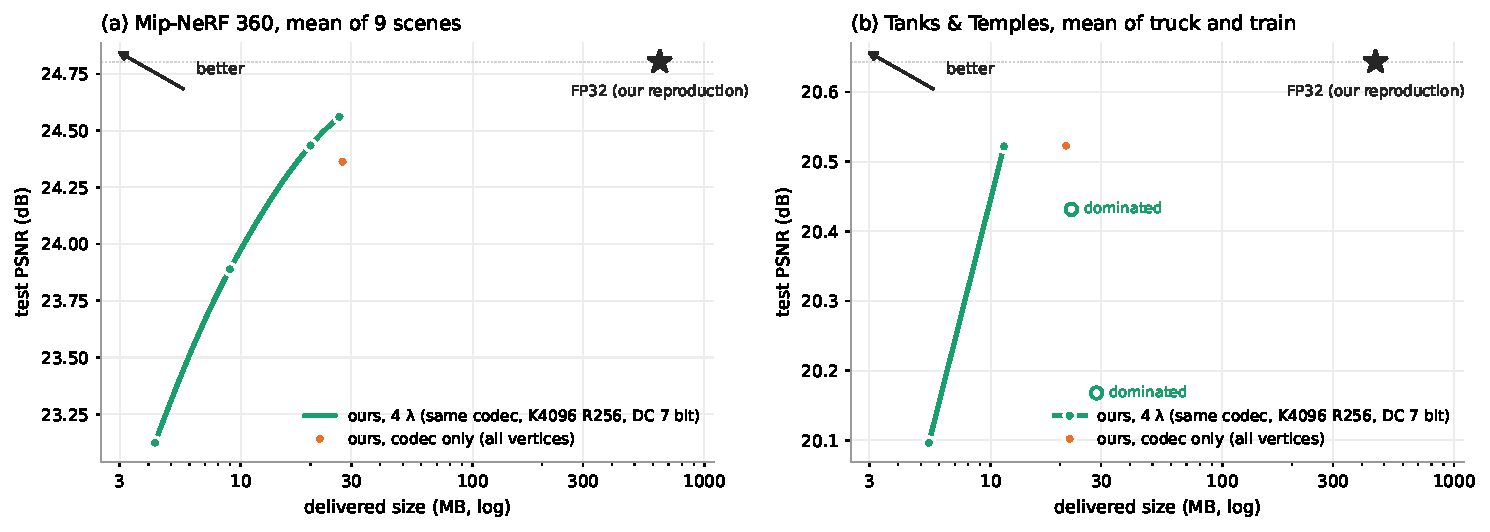
\includegraphics[width=\linewidth]{figures/fig-mean-rd-v1.pdf}
\caption{Dataset-mean RD curves behind Table~\ref{tab:headline}: the four $\lambda$ points (same codec, K4096 + R256, DC 7 bit), the codec-only point (all vertices kept) and the FP32 model. On T\&T the two smallest-$\lambda$ points are dominated (hollow): see Section~\ref{sec:perscene}.}
\label{fig:meanrd}
\end{figure}

\begin{table}[h]
\centering\small
\caption{Dataset means: Mip-NeRF~360 (9 scenes) and Tanks \& Temples (truck, train). $\Delta$PSNR is against the dataset's own FP32 row.}
\label{tab:headline}
\begin{tabular}{@{}llrrlr@{}}
\toprule
dataset & point & MB & ratio & PSNR / SSIM / LPIPS & $\Delta$PSNR vs FP32 \\
\midrule
Mip-NeRF 360 & FP32 (our reproduction) & 642 & 1$\times$ & 24.81 / 0.731 / 0.309 & -- \\
 & $\lambda = 6.2\times10^{-4}$ & 26.6 & 24$\times$ & 24.56 / 0.717 / 0.385 & $-0.24$ \\
 & $\lambda = 1.85\times10^{-3}$ & 20.0 & 32$\times$ & 24.44 / 0.709 / 0.405 & $-0.37$ \\
 & $\lambda = 6.2\times10^{-3}$ & 9.0 & 72$\times$ & 23.89 / 0.672 / 0.464 & $-0.92$ \\
 & $\lambda = 1.85\times10^{-2}$ & 4.3 & 151$\times$ & 23.12 / 0.624 / 0.518 & $-1.68$ \\
\midrule
Tanks \& Temples & FP32 (our reproduction) & 459 & 1$\times$ & 20.64 / 0.760 / 0.272 & -- \\
 & $\lambda = 6.2\times10^{-4}$ (dominated) & 28.7 & 16$\times$ & 20.17 / 0.737 / 0.332 & $-0.47$ \\
 & $\lambda = 1.85\times10^{-3}$ (dominated) & 22.3 & 21$\times$ & 20.43 / 0.745 / 0.331 & $-0.21$ \\
 & $\lambda = 6.2\times10^{-3}$ & 11.4 & 40$\times$ & 20.52 / 0.737 / 0.358 & $-0.12$ \\
 & $\lambda = 1.85\times10^{-2}$ & 5.4 & 85$\times$ & 20.10 / -- / -- & $-0.54$ \\
\bottomrule
\end{tabular}
\end{table}

\subsection{Per scene}
\label{sec:perscene}

\begin{table}[h]
\centering\scriptsize
\caption{Per scene: FP32 model and the four $\lambda$ points. Each cell is (MB (ratio), $\Delta$PSNR vs the scene's FP32 row).}
\label{tab:perscene}
\setlength{\tabcolsep}{4pt}
\resizebox{\linewidth}{!}{%
\begin{tabular}{@{}lrrllll@{}}
\toprule
scene & FP32 MB & FP32 PSNR & $\lambda\,6.2\mathrm{e}{-4}$ & $\lambda\,1.85\mathrm{e}{-3}$ & $\lambda\,6.2\mathrm{e}{-3}$ & $\lambda\,1.85\mathrm{e}{-2}$ \\
\midrule
room & 597 & 28.48 & (22.1 (27$\times$), $-0.23$) & (12.4 (48$\times$), $-0.46$) & (5.4 (110$\times$), $-1.18$) & (2.9 (207$\times$), $-2.10$) \\
counter & 520 & 26.48 & (20.7 (25$\times$), $-0.53$) & (13.1 (40$\times$), $-0.64$) & (6.4 (82$\times$), $-1.16$) & (3.3 (155$\times$), $-1.94$) \\
kitchen & 507 & 27.46 & (24.5 (21$\times$), $-0.37$) & (16.5 (31$\times$), $-0.57$) & (8.0 (63$\times$), $-1.49$) & (3.8 (134$\times$), $-2.84$) \\
bonsai & 678 & 28.28 & (24.3 (28$\times$), $-0.39$) & (13.2 (52$\times$), $-0.87$) & (6.1 (112$\times$), $-1.92$) & (3.5 (192$\times$), $-2.92$) \\
garden & 740 & 24.75 & (36.4 (20$\times$), $-0.02$) & (24.6 (30$\times$), $-0.25$) & (10.2 (73$\times$), $-1.10$) & (5.0 (149$\times$), $-1.97$) \\
bicycle & 680 & 23.04 & (31.6 (22$\times$), $-0.05$) & (27.0 (25$\times$), $-0.02$) & (11.9 (57$\times$), $-0.35$) & (5.2 (131$\times$), $-0.96$) \\
stump & 698 & 24.99 & (27.6 (25$\times$), $-0.18$) & (21.4 (33$\times$), $-0.28$) & (8.9 (79$\times$), $-0.87$) & (3.9 (178$\times$), $-1.78$) \\
flowers & 668 & 19.45 & (25.7 (26$\times$), $-0.43$) & (24.2 (28$\times$), $-0.38$) & (12.0 (56$\times$), $-0.24$) & (5.6 (118$\times$), $-0.61$) \\
treehill & 692 & 20.39 & (27.0 (26$\times$), $-0.08$) & (27.4 (25$\times$), $+0.06$) & (11.9 (58$\times$), $-0.01$) & (5.1 (136$\times$), $-0.09$) \\
truck & 432 & 22.39 & (27.3 (16$\times$), $-0.61$) & (19.3 (22$\times$), $-0.19$) & (9.4 (46$\times$), $-0.02$) & (4.4 (98$\times$), $-0.75$) \\
train & 485 & 18.90 & (30.1 (16$\times$), $-0.35$) & (25.4 (19$\times$), $-0.24$) & (13.4 (36$\times$), $-0.22$) & (6.4 (76$\times$), $-0.35$) \\
\midrule
Mip-360 mean (9) & 642 & 24.81 & (26.6 (24$\times$), $-0.25$) & (20.0 (32$\times$), $-0.37$) & (9.0 (72$\times$), $-0.92$) & (4.3 (151$\times$), $-1.69$) \\
T\&T mean (2) & 459 & 20.64 & (28.7 (16$\times$), $-0.47$) & (22.3 (21$\times$), $-0.21$) & (11.4 (40$\times$), $-0.12$) & (5.4 (85$\times$), $-0.54$) \\
\bottomrule
\end{tabular}}
\end{table}

At $\lambda = 6.2\times10^{-3}$ the same price stops growth at 5.4--8.0\,MB on the indoor scenes and 8.9--13.4\,MB outdoors: the byte budget is an outcome of the scene content, not a preset cap. On flowers, treehill, truck and train the two smallest-$\lambda$ points are dominated (a larger asset with no higher test PSNR): $\Delta D_t$ measures training-view error, and on these sparsely covered scenes the extra triangles reduce it without improving the test views (validation PSNR rises by 0.5--1.2\,dB, test by $\leq 0.2$). The Pareto hull is drawn through the non-dominated points. Section~\ref{sec:ablation} shows the complementary fact: at equal vertex count, choosing the triangles in the loop beats choosing them afterwards.

\subsection{Same asset, different codecs}
\label{sec:codecs}

\begin{figure}[h]
\centering
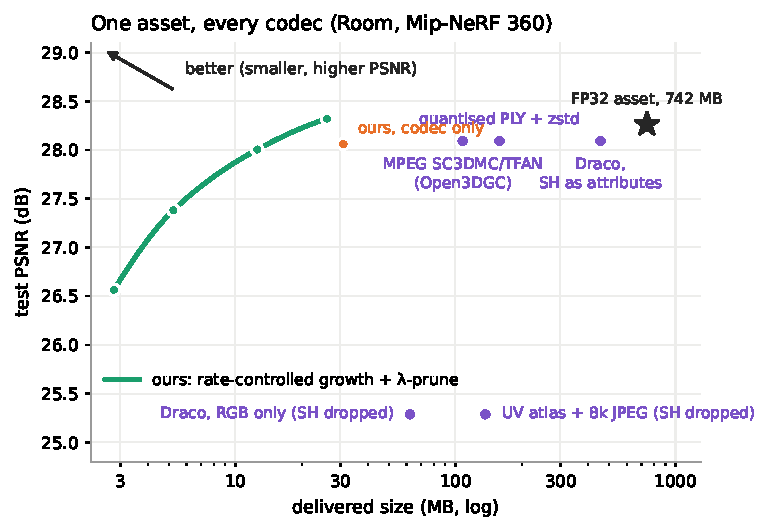
\includegraphics[width=0.9\linewidth]{figures/fig-codecs-room-v2.pdf}
\caption{One FP32 Room asset (3.19\,M vertices, 742\,MB) through generic codecs and through ours. Every point is the same trained model; only the codec differs.}
\label{fig:codecs}
\end{figure}

\begin{table}[h]
\centering\small
\caption{Room, same FP32 asset, different routes.}
\label{tab:codecs}
\resizebox{\linewidth}{!}{%
\begin{tabular}{@{}lrrl@{}}
\toprule
route & MB & PSNR & note \\
\midrule
PLY + zstd & 158.5 & 28.09 & lossless after 8-bit SH quantisation \\
MPEG SC3DMC/TFAN (Open3DGC), SH as 8-bit attributes & 108.0 & $\approx$28.09 & strongest generic row; geometry 19.9 + SH 88.1 \\
Draco, SH as attributes & 456.1 & 28.09 & splits vertices 4.5$\times$ \\
MPEG or Draco geometry + JPEG texture (4k / 8k atlas) & 91--146 & 25.3 & SH dropped, $-3.0$\,dB \\
ours, codec only (level 1.0, no growth control) & 30.9 & 28.06 & 3.5$\times$ smaller than MPEG \\
ours, $\lambda = 2\times10^{-3}$ & 13.7 & 27.99 & 7.9$\times$ smaller than MPEG \\
\bottomrule
\end{tabular}}
\end{table}

Of the 108 $\to$ 31\,MB gain, about 73\,MB comes from replacing per-vertex SH by dictionary indices and about 4\,MB from our geometry streams: keeping our SH streams and replacing only our position + connectivity streams by MPEG SC3DMC/TFAN (19.9\,MB vs our 16\,MB) makes the file 13\,\% larger. The 108\,MB row is MPEG end to end, with the SH coefficients as 8-bit attributes (88\,MB). Figure~\ref{fig:codecs} uses the 10/24 Room asset (trained without \texttt{--indoor}); every row in it is on that one asset, so it is internally consistent. Garden behaves the same way (MPEG 126\,MB vs ours 32.5\,MB at equal quality).

\subsection{Against other methods}

\begin{figure}[h]
\centering
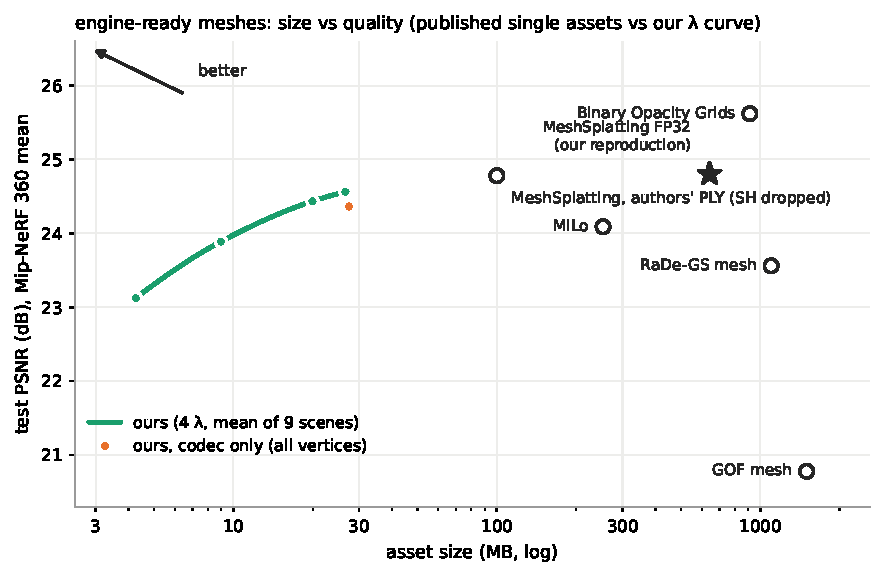
\includegraphics[width=0.8\linewidth]{figures/fig-mesh-class-v3.pdf}
\caption{Engine-ready mesh methods, Mip-NeRF~360 means: size vs PSNR. Every published point is that method's own reported single asset (Table~\ref{tab:cross-mesh}); none of them offers a rate control, so each has one point and ours is the only curve. The top-right point is Binary Opacity Grids (913\,MB, 25.62\,dB), which no opaque mesh of this class reaches at any size.}
\label{fig:mesh}
\end{figure}


\begin{table}[t]
\centering\scriptsize
\caption{Cross-method comparison, dataset means, engine-ready mesh methods. Published numbers verbatim; FPS as reported, hardware differs by row; ``--'' = not reported. $\dagger$ pipeline LPIPS convention, $\approx 0.03$ higher than the 3DGS convention of the other rows. $^{a}$ RGB-only PLY, SH dropped. $^{b}$ plus a CPU decode of 2--6\,s; FPS measured on Room (iPhone 17 Pro / MacBook Pro M2 Max, WebGL2).}
\label{tab:cross-mesh}
\setlength{\tabcolsep}{4pt}
\resizebox{\linewidth}{!}{%
\begin{tabular}{@{}llrlrl@{}}
\toprule
method & Mip-360 PSNR / SSIM / LPIPS & MB & T\&T PSNR / SSIM / LPIPS & MB & FPS \\
\midrule
MeshSplatting, paper (2025) & 24.78 / 0.728 / 0.310 & 100$^{a}$ & 20.52 / 0.745 / 0.287 & -- & 220 / 190 (M4) \\
MeshSplatting FP32, our reproduction & 24.81 / 0.731 / 0.309 & 642 & 20.64 / 0.760 / 0.272 & 459 & -- \\
MiLo (SIGGRAPH Asia 2025) & 24.09 / 0.688 / 0.323 & 253 & 21.46 / 0.706 / 0.348 & -- & 170 / 160 (M4) \\
Binary Opacity Grids (SIGGRAPH 2024) & 25.62 / -- / -- & 913 & -- & -- & 927 (desktop) \\
RaDe-GS mesh (2024) & 23.56 / 0.668 / 0.361 & 1100 & 20.51 / 0.659 / 0.344 & -- & OOM on M4 \\
GOF mesh (2024) & 20.78 / 0.573 / 0.465 & 1500 & 21.69 / 0.690 / 0.326 & -- & OOM on M4 \\
\midrule
\textbf{ours, $\lambda = 6.2\times10^{-4}$} & 24.56 / 0.717 / 0.385$^\dagger$ & 26.6 & 20.17 / 0.737 / 0.332$^\dagger$ & 28.7 & 350 phone / 820 laptop$^{b}$ \\
\textbf{ours, $\lambda = 1.85\times10^{-3}$} & 24.44 / 0.709 / 0.405$^\dagger$ & 20.0 & 20.43 / 0.745 / 0.331$^\dagger$ & 22.3 & 350 phone / 820 laptop$^{b}$ \\
\textbf{ours, $\lambda = 6.2\times10^{-3}$} & 23.89 / 0.672 / 0.464$^\dagger$ & 9.0 & 20.52 / 0.737 / 0.358$^\dagger$ & 11.4 & 350 phone / 820 laptop$^{b}$ \\
\bottomrule
\end{tabular}}
\end{table}


Inside the engine-ready mesh class we reach MiLo's quality at 22$\times$ fewer bytes, RaDe-GS's at 175$\times$, GOF's at 352$\times$ with $+2.3$\,dB; the authors' own RGB-only PLY (100\,MB) is 4$\times$ larger than our best point and 0.22\,dB higher only because it drops SH entirely. Against 3DGS-class codecs our absolute PSNR is about 3\,dB lower; this is the opaque-mesh representation gap, present already in uncompressed MeshSplatting (2.7\,dB below 3DGS), not a codec gap. Published mesh methods do not compare against Gaussian codecs, and neither does the main text; the numbers are in Appendix~\ref{app:gauss} for reference.

\subsection{Ablation: is the rate in the loop worth it?}
\label{sec:ablation}

\begin{figure}[h]
\centering
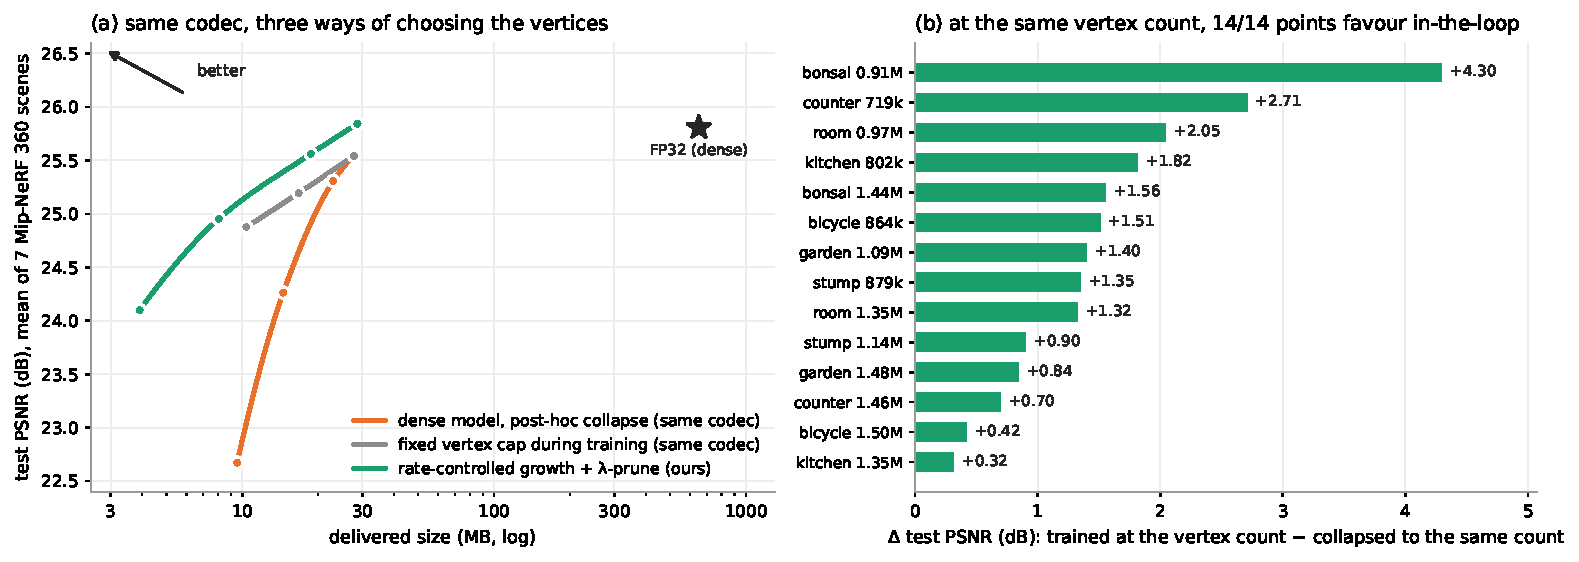
\includegraphics[width=\linewidth]{figures/fig-in-the-loop-v1.pdf}
\caption{Same codec, three ways of choosing vertices (7 Mip-NeRF~360 scenes, older parameter set): post-hoc edge collapse, fixed vertex cap, $\lambda$-growth + prune. (b) At equal vertex count the in-the-loop choice wins on 14 of 14 points.}
\label{fig:loop}
\end{figure}

With the codec held fixed, post-hoc edge collapse to 10\,MB falls to 22.7\,dB mean, training under a fixed vertex cap reaches 24.9\,dB, and $\lambda$-priced growth plus prune reaches 25.0\,dB and keeps going down to 4\,MB. At matched vertex count the in-the-loop choice wins on every scene, by $+0.3$ to $+4.3$\,dB. The prune rounds alone are a small effect ($-8$\,\% bytes at $+0.01$--$0.02$\,dB on Room); the gain is in where growth is allowed to happen.

\subsection{Deployability}

\begin{table}[h]
\centering\small
\caption{Deployability at the $\lambda = 6.2\times10^{-3}$ point. Laptop = MacBook Pro M2 Max (Chrome), phone = iPhone 17 Pro (Safari), WebGL2 viewer, SH degree 3, full capture resolution.}
\label{tab:deploy}
\resizebox{\linewidth}{!}{%
\begin{tabular}{@{}lrrlrll@{}}
\toprule
scene & asset MB & ratio & train min, upstream $\to$ ours & CPU decode s (1 core) & laptop ms (fps) & phone ms (fps) \\
\midrule
room & 5.2 & 142$\times$ & 51 $\to$ 27 (0.52$\times$) & 2.3 & 1.2 (820) & 2.8 (352) \\
garden & 10.2 & 73$\times$ & 49 $\to$ 24 (0.48$\times$) & 4.4 & 1.8 (566) & 6.3 (160) \\
bicycle & 11.9 & 57$\times$ & 41 $\to$ 25 (0.60$\times$) & 5.4 & 1.9 (523) & 6.9 (145) \\
\midrule
11-scene mean & 9.4 & 73$\times$ & 0.57$\times$ & 4.1 & -- & -- \\
\bottomrule
\end{tabular}}
\end{table}

Training takes $0.57\times$ the upstream time because the priced growth stops at fewer triangles and the rasteriser's cost scales with their number; nothing else in the optimisation changed. The decoder is a standalone single-core program with no access to the training data.

\subsection{Joint $\lambda \times$ dictionary-size traversal}
\label{sec:fan}

The $\lambda$ curve above is traced at one delivery setting (K4096 + R256, DC 7 bit) chosen on post-hoc vertex levels of Room (Appendix~\ref{app:levels}). To check that this setting stays on the joint hull, every $\lambda$ asset of room, kitchen and garden is re-exported, without training, with four other dictionaries ($K\times R \in \{4096\times1,\ 1024\times256,\ 4096\times1024,\ 16384\times1024\}$; $k$-means re-fit and the 400-step bank refit on the same mesh) and with DC at 8 bits: 24 points per scene, Table~\ref{tab:fan} and Figure~\ref{fig:fan}.

\begin{table}[h]
\centering\scriptsize
\caption{$\lambda \times$ dictionary fan. First number column: the delivered K4096 + R256 + DC 7-bit asset (MB / test PSNR). Every other cell: $\Delta$MB / $\Delta$PSNR of the re-export against that row's delivered asset.}
\label{tab:fan}
\resizebox{\linewidth}{!}{%
\begin{tabular}{@{}lrrrrrr@{}}
\toprule
scene, $\lambda$ & delivered & DC 8 bit & K4096 R1 & K1024 R256 & K4096 R1024 & K16384 R1024 \\
\midrule
room, 6.2e-4 & 22.07 / 28.255 & +0.94 / +0.066 & -1.95 / -0.172 & -1.01 / -0.107 & +0.60 / +0.034 & +3.01 / +0.084 \\
room, 1.85e-3 & 12.40 / 28.023 & +0.50 / +0.065 & -1.05 / -0.180 & -0.75 / -0.104 & +0.38 / +0.031 & +2.50 / +0.087 \\
room, 6.2e-3 & 5.40 / 27.305 & +0.18 / +0.105 & -0.44 / -0.164 & -0.57 / -0.071 & +0.22 / +0.026 & +2.15 / +0.077 \\
room, 1.85e-2 & 2.89 / 26.383 & +0.09 / +0.069 & -0.22 / -0.145 & -0.50 / -0.071 & +0.16 / +0.024 & +2.00 / +0.072 \\
kitchen, 6.2e-4 & 24.46 / 27.092 & +0.97 / +0.038 & -1.84 / -0.330 & -0.96 / -0.157 & +0.56 / +0.062 & +2.93 / +0.162 \\
kitchen, 1.85e-3 & 16.54 / 26.886 & +0.62 / +0.039 & -1.22 / -0.326 & -0.79 / -0.153 & +0.39 / +0.059 & +2.57 / +0.163 \\
kitchen, 6.2e-3 & 8.02 / 25.971 & +0.27 / +0.035 & -0.58 / -0.307 & -0.61 / -0.142 & +0.24 / +0.056 & +2.24 / +0.154 \\
kitchen, 1.85e-2 & 3.78 / 24.623 & +0.12 / +0.036 & -0.28 / -0.249 & -0.52 / -0.115 & +0.17 / +0.048 & +2.06 / +0.131 \\
garden, 6.2e-4 & 36.39 / 24.734 & +1.65 / +0.016 & -3.12 / -0.113 & -1.38 / -0.035 & +0.88 / +0.019 & +3.62 / +0.043 \\
garden, 1.85e-3 & 24.60 / 24.504 & +1.09 / +0.017 & -2.08 / -0.110 & -1.07 / -0.034 & +0.62 / +0.019 & +3.04 / +0.040 \\
garden, 6.2e-3 & 10.18 / 23.650 & +0.41 / +0.014 & -0.84 / -0.102 & -0.70 / -0.033 & +0.31 / +0.020 & +2.37 / +0.037 \\
garden, 1.85e-2 & 4.97 / 22.783 & +0.18 / +0.015 & -0.40 / -0.089 & -0.57 / -0.025 & +0.20 / +0.015 & +2.14 / +0.029 \\
\bottomrule
\end{tabular}}
\end{table}

\begin{figure}[h]
\centering
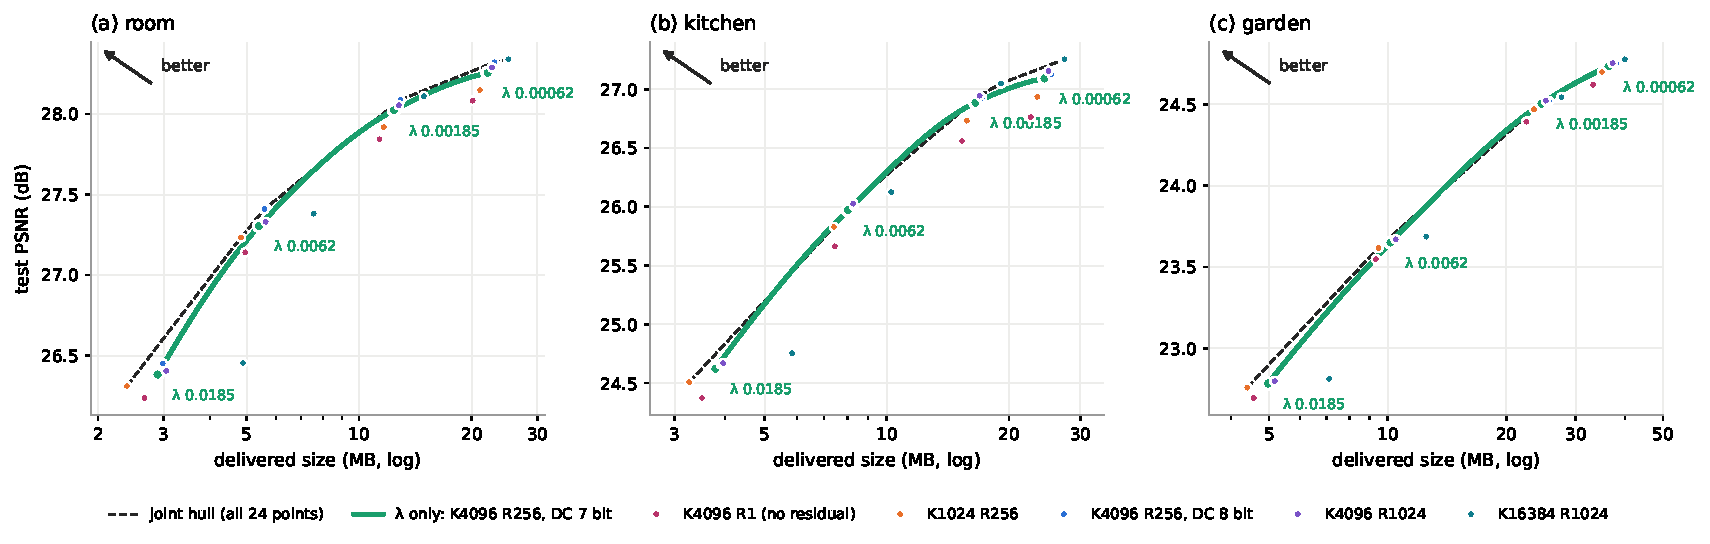
\includegraphics[width=\linewidth]{figures/fig-fan-v1.pdf}
\caption{The same 72 points: the $\lambda$-only curve (green, the delivered setting), the five re-exports at every $\lambda$, and the joint hull over all 24 points of a scene (dashed).}
\label{fig:fan}
\end{figure}

Three readings. (i) \textbf{The fixed setting is within 0.1\,dB of the joint hull everywhere.} At the bytes of each delivered asset the joint hull is higher by 0.00--0.05\,dB on garden, 0.00--0.09 on kitchen and 0.02--0.12 on room; the $\lambda$ lever (moving to the neighbouring asset, 0.02--0.37\,dB per MB) is cheaper than or equal to every dictionary lever at all 12 points except the ones named next. (ii) \textbf{Where the hull leaves the setting, it does so in one direction per rate.} At the low-rate end ($\lambda = 1.85\times10^{-2}$, 3--5\,MB) the smaller main bank K1024 is on every hull (0.04--0.22\,dB per MB saved against a $\lambda$ chord of 0.17--0.37); at the high-rate end ($\lambda \le 1.85\times10^{-3}$, $\ge 17$\,MB) the larger dictionaries K4096 R1024 and K16384 R1024 are on the kitchen and garden hulls (0.03--0.15\,dB per MB against a chord of 0.02--0.03). Dictionary size should grow with the vertex count, roughly $K \propto V$; a rule of that form is a one-line change in the exporter and is left for the camera-ready. The residual bank is never dropped: K4096 R1 is the most expensive cut at every point (0.09--0.90\,dB per MB). (iii) \textbf{DC precision is scene-dependent.} 8-bit DC costs the same $\approx 3$\,bit per vertex everywhere but returns 0.07--0.10\,dB on room against 0.01--0.04 on kitchen and garden; on room it is on the joint hull at three of the four $\lambda$. Within the 0.1\,dB band none of these choices changes the headline or the ordering against other methods; they are the allocator's second-order decisions, priced by the same slopes as the vertices.

\subsection{Where the top-rate loss on the indoor models comes from}
\label{sec:indoor}

The delivered level-1.0 assets of the \texttt{--indoor} models lose 0.49 (room) and 0.76\,dB (kitchen) against FP32; 0.11 / 0.14 of it is the 3000-step geometry finetune and the rest, 0.38 / 0.62\,dB, the SH dictionary + quantisation chain. Table~\ref{tab:indoor} opens that chain on the same finetuned meshes without training: every exporter setting is relaxed one at a time, and the exporter's own stage log (validation PSNR after $k$-means assignment, after the bank refit and after decoding) separates the sharing loss from the quantisation loss.

\begin{table}[h]
\centering\scriptsize
\caption{Top-rate loss decomposition on the \texttt{--indoor} room and kitchen deliveries (all vertices, K4096 + R256, DC 7 bit, XYZ q14 / q16). Left: one setting relaxed per row, test PSNR change and bytes. Right: the exporter's stage log on validation views, validation PSNR relative to the finetuned mesh after $k$-means assignment, after the 400-step bank refit and after decoding; sharing = refit, quant. = decoded $-$ refit.}
\label{tab:indoor}
\resizebox{\linewidth}{!}{%
\begin{tabular}{@{}llrrr@{}}
\toprule
scene & setting relaxed & MB & $\Delta$PSNR & dB / MB \\
\midrule
room & delivered (25.74\,MB, 27.994\,dB) & 25.74 & -- & -- \\
room & DC 8 bit & 26.86 & $+0.077$ & 0.068 \\
room & per-vertex opacity instead of one scalar & 28.11 & $+0.000$ & 0.000 \\
room & XYZ q15 & 26.70 & $+0.082$ & 0.085 \\
room & XYZ q16 & 27.65 & $+0.106$ & 0.055 \\
room & K4096 R1024 & 26.44 & $+0.035$ & 0.049 \\
room & K16384 R1024 & 28.98 & $+0.090$ & 0.028 \\
\midrule
kitchen & delivered (24.33\,MB, 26.706\,dB) & 24.33 & -- & -- \\
kitchen & DC 8 bit & 25.41 & $+0.043$ & 0.040 \\
kitchen & per-vertex opacity instead of one scalar & 26.56 & $+0.000$ & 0.000 \\
kitchen & K4096 R1024 & 24.93 & $+0.068$ & 0.113 \\
kitchen & K16384 R1024 & 27.35 & $+0.181$ & 0.060 \\
\bottomrule
\end{tabular}%
\hspace{1em}%
\begin{tabular}{@{}llrrrr@{}}
\toprule
scene & dictionary & after $k$-means & after refit & decoded & sharing / quant. \\
\midrule
room & K4096 R256 & $-1.07$ & $-0.47$ & $-0.82$ & $-0.47$ / $-0.35$ \\
room & K4096 R1024 & $-0.94$ & $-0.40$ & $-0.75$ & $-0.40$ / $-0.35$ \\
room & K16384 R1024 & $-0.73$ & $-0.29$ & $-0.64$ & $-0.29$ / $-0.36$ \\
\midrule
kitchen & K4096 R256 & $-1.22$ & $-0.73$ & $-0.85$ & $-0.73$ / $-0.12$ \\
kitchen & K4096 R1024 & $-1.09$ & $-0.64$ & $-0.77$ & $-0.64$ / $-0.13$ \\
kitchen & K16384 R1024 & $-0.88$ & $-0.51$ & $-0.64$ & $-0.51$ / $-0.13$ \\
\bottomrule
\end{tabular}}
\end{table}

The loss is distributed, and no single quantiser causes it. On kitchen 85\,\% of it is the SH sharing itself (per-vertex SH replaced by dictionary codes, $-0.73$\,dB on validation after the refit); a 16$\times$ larger main bank recovers 0.22\,dB of it for 12\,\% more bytes, and the DC and position quantisers together cost 0.12\,dB. On room the sharing and the quantisers split the loss about evenly; of the quantiser half, DC 7 bit accounts for 0.08\,dB and the XYZ grid for 0.08--0.11 (the precision rule of Section~\ref{sec:codec} is one bit conservative on this model, as it was on three of the seven scenes measured on post-hoc levels). The single opacity scalar costs nothing on either model while saving 2.2--2.4\,MB. The 400-step bank refit is what makes dictionary sharing viable at all: it recovers 0.4--0.6\,dB of the raw $k$-means assignment loss on every row. The \texttt{--indoor} models share colour less well than the default ones (their per-vertex SH has a larger learning rate and fewer vertices carry more colour variance), which is why the same fixed setting loses 0.2 more dB on them; the remedy is the rate-dependent dictionary of Section~\ref{sec:fan}, not a different quantiser. Each remaining lever buys 0.03--0.18\,dB for 4--12\,\% of the file, i.e.\ the top-rate ceiling is a property of the hull, priced by the same slopes as every other choice.

\subsection{What is still open}
\begin{itemize}[nosep,leftmargin=*]
  \item The byte prices are a calibrated constant proxy for the rate; a context-dependent (trainable) rate model would make $B_a$ a function of the local neighbourhood. We report the sensitivity of the operating point to the constants (Section~\ref{sec:rate}) and leave the trainable model as future work.
  \item The $\lambda \times$ dictionary fan on the remaining eight scenes ($\approx 12$\,GPU-h), a rate-dependent dictionary rule ($K \propto V$) and the one-bit XYZ margin are exporter-side changes within the 0.1\,dB band of Section~\ref{sec:fan}; they will be applied in one pass with the unified LPIPS evaluation ($\approx 3$\,GPU-h). MPEG rows for the remaining nine scenes (CPU) are pending; none of these changes the ordering above.
\end{itemize}

\appendix
\section{Dictionary size on post-hoc vertex levels}
\label{app:levels}
On Room the $K \times R$ sweep was run at four vertex levels (100, 80, 70, 50\,\% of the dense mesh, 12 dictionaries each) and on six scenes at one level; a greedy allocator over the three levers (vertices, dictionary, precision) reproduces the global Room hull on 9 of 9 points. Near the chosen setting every lever costs 0.02--0.06\,dB per MB: K4096 R256 $\to$ R1024 buys 0.022\,dB per MB, DC 7 $\to$ 8 bit 0.022, K16384 0.014--0.020; the frontier is smooth and no single knob dominates, which is why one setting is used for every $\lambda$ and Table~\ref{tab:fan} checks it on the $\lambda$ assets themselves.

\section{3DGS-class methods, for reference}
\label{app:gauss}
\begin{figure}[h]
\centering
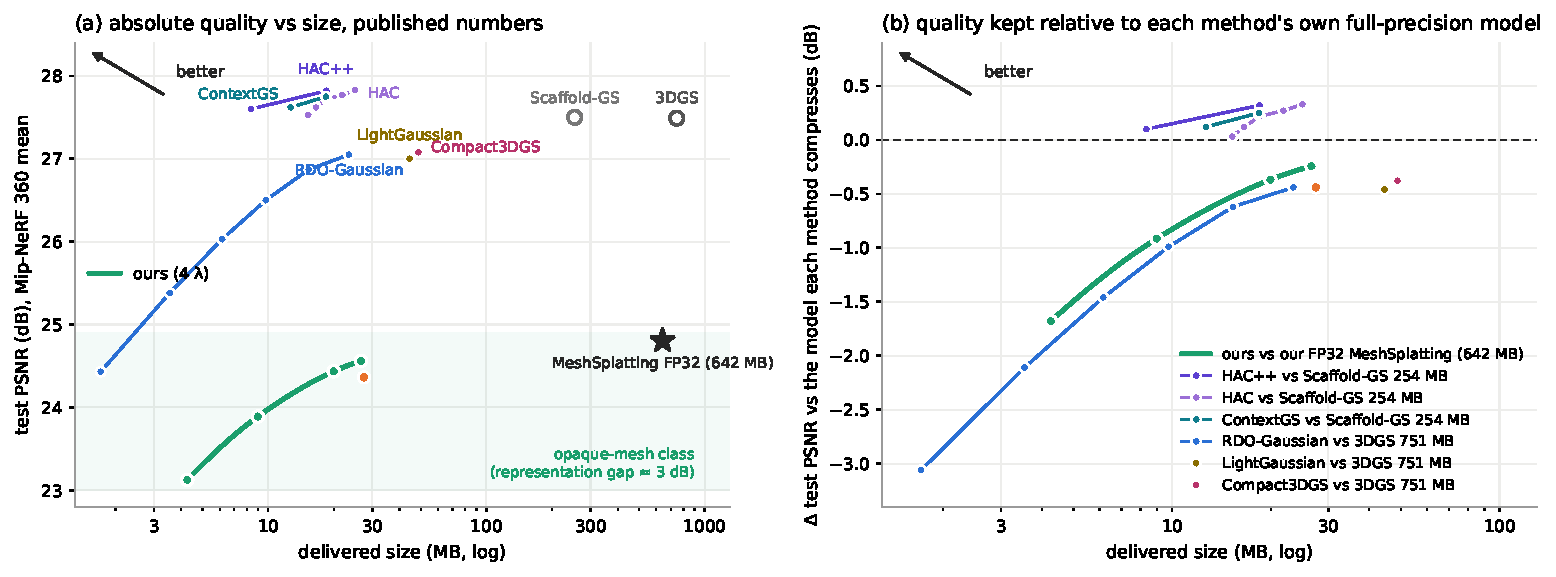
\includegraphics[width=\linewidth]{figures/fig-gauss-class-v2.pdf}
\caption{3DGS-class codecs. (a) absolute numbers; (b) quality retained relative to each method's own full-precision model.}
\label{fig:gauss}
\end{figure}

\begin{table}[t]
\centering\scriptsize
\caption{Cross-method comparison, dataset means, 3DGS-class methods (not engine-ready meshes). Published numbers verbatim; FPS as reported, hardware differs by row; ``--'' = not reported. Ours (Table~\ref{tab:cross-mesh}) is $\approx 3$\,dB below this class in absolute PSNR; this is the opaque-mesh representation gap, present already in uncompressed MeshSplatting.}
\label{tab:cross-3dgs}
\setlength{\tabcolsep}{4pt}
\resizebox{\linewidth}{!}{%
\begin{tabular}{@{}llrlrl@{}}
\toprule
method & Mip-360 PSNR / SSIM / LPIPS & MB & T\&T PSNR / SSIM / LPIPS & MB & FPS \\
\midrule
3DGS (SIGGRAPH 2023) & 27.46 / 0.812 / 0.222 & 750.9 & 23.69 / 0.844 / 0.178 & 431.0 & 99 (desktop) \\
Scaffold-GS (CVPR 2024) & 27.50 / 0.806 / 0.252 & 253.9 & 23.96 / 0.853 / 0.177 & 86.5 & 135 \\
HAC++ low (2025) & 27.60 / 0.803 / 0.253 & 8.34 & 24.22 / 0.849 / 0.190 & 5.18 & 130--151 \\
HAC++ high (2025) & 27.82 / 0.811 / 0.231 & 18.48 & 24.32 / 0.854 / 0.178 & 8.63 & 130--151 \\
RDO-Gaussian (ECCV 2024) & 27.05 / 0.802 / 0.239 & 23.46 & 23.34 / 0.835 / 0.195 & 12.03 & -- \\
Compact3DGS (CVPR 2024) & 27.08 / 0.798 / 0.247 & 48.80 & 23.32 / 0.831 / 0.201 & 39.43 & -- \\
LightGaussian (NeurIPS 2024) & 27.00 / 0.799 / 0.249 & 44.54 & 22.83 / 0.822 / 0.242 & 22.43 & -- \\
\bottomrule
\end{tabular}}
\end{table}

\begin{thebibliography}{9}
\bibitem{witten1987} I.~H. Witten, R.~M. Neal, J.~G. Cleary. Arithmetic coding for data compression. \emph{Comm. ACM} 30(6), 1987.
\bibitem{deering1995} M. Deering. Geometry compression. \emph{SIGGRAPH} 1995.
\bibitem{touma1998} C. Touma, C. Gotsman. Triangle mesh compression. \emph{Graphics Interface} 1998.
\bibitem{draco} Google. Draco 3D data compression. \url{https://github.com/google/draco}.
\bibitem{zstd} Y. Collet, M. Kucherawy. Zstandard compression and the application/zstd media type. RFC 8878, 2021.
\end{thebibliography}

\end{document}
